\begin{figure}[t]
\centering
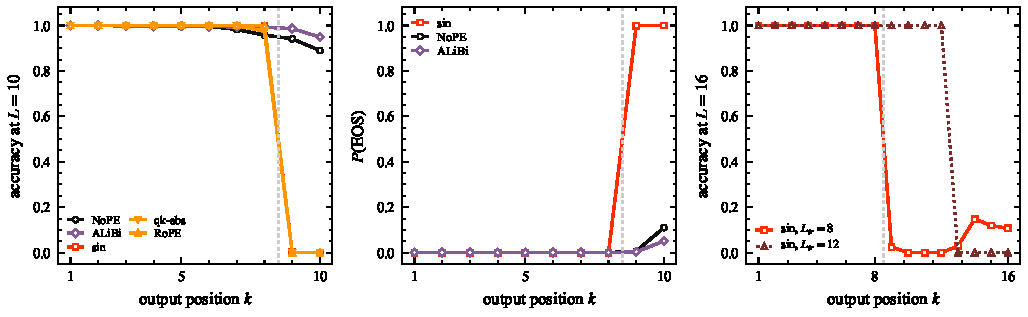
\includegraphics[width=\textwidth]{../figures/fig_profile.pdf}
\caption{The failure is a stop. (a) Accuracy at each output position, copy, test
length $10$, $L_{\mathrm{tr}}{=}8$. Sin, $q/k$-absolute and rotary are correct at
every position up to the eighth and wrong from the ninth; \nope{} and ALiBi decay
gently. The vertical line marks $L_{\mathrm{tr}}$. (b) Probability assigned to EOS
at the same positions: $1.00$ from the ninth for sin, below $0.1$ throughout for
\nope{} and ALiBi. (c) The boundary follows the training length: with
$L_{\mathrm{tr}}{=}12$ the same code is correct to the twelfth position at
$L{=}16$, and at $L{=}8$ it truncates at the eighth. Means over two seeds except
(c)'s $L_{\mathrm{tr}}{=}12$ run, which is a single run.}
\label{fig:profile}
\end{figure}
